\documentclass[review,draft,12pt]{elsarticle}
%\documentclass[12pt,draft]{article}
\usepackage{amsmath, amsfonts, amssymb}  % extended mathematics
\usepackage{ifxetex}
\ifxetex
  \usepackage{fontspec,xltxtra,xunicode}
  \defaultfontfeatures{Mapping=tex-text,Scale=MatchLowercase}
  \setmainfont{TeX Gyre Pagella}
  \setsansfont{Cabin}
  \setmonofont{Bitstream Vera Sans Mono}
\else
  \usepackage[mathletters]{ucs}
  \usepackage[utf8x]{inputenc}
\fi

% My package additions
\usepackage[hyphens]{url}
\usepackage{lineno} % add 
\usepackage{longtable}
\usepackage{lscape}
%\usepackage{setspace}
\linenumbers % turns line numbering on 
\usepackage{natbib}
\bibliographystyle{elsarticle-num}
%\bibliographystyle{abbrvnat}
\biboptions{sort&compress} % For natbib
\usepackage{graphicx}
\usepackage{booktabs} % book-quality tables
\usepackage{ifdraft}
\usepackage{caption}
\usepackage{subscript}
\usepackage{textcomp}

% A modified page layout
\textwidth 6.75in
\oddsidemargin -0.15in
\evensidemargin -0.15in
\textheight 9in
\topmargin -0.5in


\usepackage{microtype}
\usepackage{fancyhdr}
\pagestyle{fancy}
\pagenumbering{arabic}

\usepackage{listings}
\lstnewenvironment{code}{\lstset{language=Haskell,basicstyle=\small\ttfamily}}{}


\setlength{\parindent}{0pt}
\setlength{\parskip}{6pt plus 2pt minus 1pt}


%%% Syntax Highlighting for code  %%%
%%% Adapted from knitr book %%% 
\usepackage{fancyvrb}
\DefineVerbatimEnvironment{Highlighting}{Verbatim}{commandchars=\\\{\}}
% Add ',fontsize=\small' for more characters per line
\newenvironment{Shaded}{}{}
\newcommand{\KeywordTok}[1]{\textcolor[rgb]{0.00,0.44,0.13}{\textbf{{#1}}}}
\newcommand{\DataTypeTok}[1]{\textcolor[rgb]{0.56,0.13,0.00}{{#1}}}
\newcommand{\DecValTok}[1]{\textcolor[rgb]{0.25,0.63,0.44}{{#1}}}
\newcommand{\BaseNTok}[1]{\textcolor[rgb]{0.25,0.63,0.44}{{#1}}}
\newcommand{\FloatTok}[1]{\textcolor[rgb]{0.25,0.63,0.44}{{#1}}}
\newcommand{\CharTok}[1]{\textcolor[rgb]{0.25,0.44,0.63}{{#1}}}
\newcommand{\StringTok}[1]{\textcolor[rgb]{0.25,0.44,0.63}{{#1}}}
\newcommand{\CommentTok}[1]{\textcolor[rgb]{0.38,0.63,0.69}{\textit{{#1}}}}
\newcommand{\OtherTok}[1]{\textcolor[rgb]{0.00,0.44,0.13}{{#1}}}
\newcommand{\AlertTok}[1]{\textcolor[rgb]{1.00,0.00,0.00}{\textbf{{#1}}}}
\newcommand{\FunctionTok}[1]{\textcolor[rgb]{0.02,0.16,0.49}{{#1}}}
\newcommand{\RegionMarkerTok}[1]{{#1}}
\newcommand{\ErrorTok}[1]{\textcolor[rgb]{1.00,0.00,0.00}{\textbf{{#1}}}}
\newcommand{\NormalTok}[1]{{#1}}
\usepackage{enumerate}
%\usepackage{ctable}
\usepackage{float}



%% Redefines the elsarticle footer
\makeatletter
\def\ps@pprintTitle{%
 \let\@oddhead\@empty
 \let\@evenhead\@empty
 \def\@oddfoot{\it \hfill\today}%
 \let\@evenfoot\@oddfoot}
\makeatother

% This is needed because raggedright in table elements redefines \\:
\newcommand{\PreserveBackslash}[1]{\let\temp=\\#1\let\\=\temp}
\let\PBS=\PreserveBackslash
\usepackage[normalem]{ulem}
\newcommand{\textsubscr}[1]{\ensuremath{_{\scriptsize\textrm{#1}}}}

% Configure hyperlinks package
\usepackage[breaklinks=true,linktocpage,pdftitle={Viral niche construction alters hosts and ecosystems at multiple scales.},pdfauthor={},colorlinks,linkcolor=blue]{hyperref}
\hypersetup{breaklinks=true, pdfborder={0 0 0}}

% Pandoc toggle for numbering sections (defaults to be off)
\setcounter{secnumdepth}{0}

% Hack to fix image sizes from pandoc and allow for suppression of figures according to TREE's requirements.
\ifdraft{\captionsetup{labelformat=empty,labelsep=none,textformat=empty}}{}
\newcounter{figureplaceholder}
\stepcounter{figureplaceholder}
\ifdraft{\renewcommand{\includegraphics}[1]{\begin{center}\fbox{Figure \arabic{figureplaceholder} about here.}\end{center}\stepcounter{figureplaceholder}}}{\let\Oldincludegraphics\includegraphics\renewcommand{\includegraphics}[1]{\Oldincludegraphics[width=0.8\textwidth]{#1}}}

\VerbatimFootnotes % allows verbatim text in footnotes

% Doublespacing
%\doublespacing


% Pandoc header



\begin{document}
\begin{frontmatter}
  \title{Viral niche construction alters hosts and ecosystems at multiple scales.}
  \author[babs]{Steven Hamblin\corref{cor1}}
  \author[babs]{Peter A. White}
  \author[babs]{Mark M. Tanaka}

  \cortext[cor1]{Corresponding author: Hamblin, S. R. (shamblin@usc.edu).  Current affiliation: Molecular and Computational Biology, 1050 Childs Way, University of Southern California, Los Angeles CA, 90089}
  \address[unsw]{School of Biotechnology and Biomolecular Sciences, University of New South Wales, Sydney, Australia 2052}
 

\begin{abstract}
The classical picture of viruses focuses on pathogenic viruses damaging the host’s cells and physiology and host-pathogen immune coevolution. However, a broader picture of viruses is emerging that includes weakly pathogenic, commensal or even mutualistic viruses and includes gross behavioural manipulations and viral effects on ecosystems. In this paper, we argue for a niche construction as unifying perspective on viral evolution. As obligate intracellular parasites, viruses are always modifying their environment, and these modifications drive evolutionary feedback between the virus and its environment across multiple scales from cells to ecosystems. We argue that niche construction will provide new insights into viral evolution, and that virology is a powerful source of empirical tests for niche construction. 
\end{abstract}

\begin{keyword}
Niche construction \sep viruses \sep host-pathogen coevolution
\end{keyword}
\end{frontmatter}

\section{Of niches and viruses}\label{of-niches-and-viruses}

The classical picture of viruses centers on a pathogenic and obligate
intracellular parasite that damages or destroys host cells and often has
detrimental effects on the host while replicating and transmitting. This
has led to a strong understanding of viruses such as influenza and human
immunodeficiency virus (HIV), and provided a wide literature of
theoretical and empirical work on viral evolution and epidemiology.
However, viruses also display a startling range of effects on hosts and
the wider environment of the host. These effects range from beneficial
mutualisms and commensalisms to behavioural manipulations and even
impacts upon global ecosystems. Such interactions with the host and its
environment are even more surprising given that viral genomes are often
compressed and lack machinery for protein synthesis.

Standard evolutionary theory can be used to provide explanations for
these phenomena but does not emphasize the process of organism-mediated
environmental changes that bias selection in viral systems. For example,
some parvoviruses contribute to host aphid survival by creating winged
morphs that aid in dispersal to neighboring plants (uninfected clones
cannot grow wings) \citep{Ryabov2009}. These winged morphs increase host
availability by allowing aphids to colonise new plants in response to
crowding and poor plant quality. The new selective pressures on viral
transmission that result can be explained as viral adaptation to an
environmental change (increased host availability), but this does not
highlight that the virus itself caused this environmental change, nor
that changes in evolutionary conditions apply to descendents far removed
from the viruses responsible for production of the dispersal morphs.
There is a growing list of viruses recognised to modify their own or
others' selection in these complex ways, but while this has been
discussed in the virological literature there has been little attempt to
comprehensively explain and even predict their occurence.

Niche construction theory (NCT; see Box 1), which can be viewed as a
generalisation of standard evolutionary theory, has the potential to
incorporate all of these effects into a single explanatory framework.
Adopting a niche construction perspective aids the study of viral
evolution by providing new insights into the causes and consequences of
viral manipulations of their host environment and beyond. Despite the
number of reserachers working on niche construction, this perspective
has not yet been applied to viruses in the evolutionary biology or
ecology literature. Conversely, one of the strongest criticisms of niche
construction is the paucity of empirical tests to date, but advances in
virology allow us to directly manipulate many aspects of viral structure
and function. Thus, we believe that viruses and niche construction need
each other: niche construction assists in explaining viral evolution,
and viruses provide a powerful platform for testing niche construction.

\begin{center}\rule{3in}{0.4pt}\end{center}

\section{Box 1: Niche construction}\label{box-1-niche-construction}

Here we provide a brief introduction to niche construction and refer the
reader to references \citep{Odling-Smee:2003fk, Odling-Smee:2013zr} for
in-depth discussion of niche construction and its relation to standard
evolutionary theory. Niche construction is defined as the ``process
whereby organisms, through their metabolism, their activities, and their
choices, modify their own and/or each other's niches''
\citep{Laland:2006pd}. By modifying biotic and abiotic sources of
selection in the their environment, organisms can modify their own
selective pressures and those of other affected organisms in a feedback
process that creates a genetic and ecological inheritance \citep[Figure
2, and see Figure 2 of][]{Odling-Smee:2013zr}. A popular example of
niche construction is the turnover and consumption of soil by earthworms
\citep{Odling-Smee:2003fk}, which changes the soil chemistry, structure,
aeration, drainage, and more. This benefits plants as earthworms enhance
the recycling of plant nutrients, and earthworms in turn benefit from
increased plant litter supply owing to increased plant growth. These
changes have accumulated over generations such that earthworms now
experience a different selective environment from that of their
ancestors. One indicator of this change is that earthworms retain
ancestral freshwater kidneys that do not show the adaptations one would
expect of a land-dwelling organism (e.g.~producing urine volumes similar
to freshwater animals) \citep{Odling-Smee:2003fk}.

Similarly, viruses can have effects on the host and beyond that will
create multigenerational effects and feed back into the selective
pressures experienced by descendant viruses. Many examples of niche
construction in viruses, such as the aggression caused by rabies, will
result in modified selection on the important viral traits of
transmission and virulence. It is important to note, though, that viral
fitness need not be increased (or even modified) for niche construction
to occur. For example, GB virus C (GBV-C) has been found to inhibit the
replication of HIV in a way that enhances the survival of the host, an
effect strong enough that the use of GBV-C is being investigated as a
potential biotherapy \citep{Gretch:2012zt}. GBV-C is vertically,
parenterally and sexually transmitted and might benefit from increased
host survival, but even if no benefit to the virus were found, the
effects on the host and the co-infecting HIV make this an example of
viral niche construction.

A challenge to the use of niche construction for viruses lies in the
broad definition of niche construction itself
\citep{Scott-Phillips2014}. Viruses are obligate intracellular parasites
and must heavily modify their host to survive; such modifications
generally lead to increased demands on the cell for energy, materials
and macro-molecular synthesis. Thus, every viral interaction with their
host could be labelled as niche construction. Following discussion in
\citep{Scott-Phillips2014}, we suggest that a practical approach to take
is to ask `when is it important or useful to emphasize the action of
niche construction'? The modifications made to a host cell when it is
used by the virus for injection and replication may meet the definition
of niche construction, but these are already well-studied by standard
theoretical and empirical approaches and need no further development in
a niche construction framework. Instead, niche construction is most
useful in analyzing interactions that extend beyond the effect of the
virus on its immediate cellular environment (the innermost layers of
Figure 1) to the physiology, behaviour, and broader environment of the
host.

\begin{figure}[htbp]
\centering
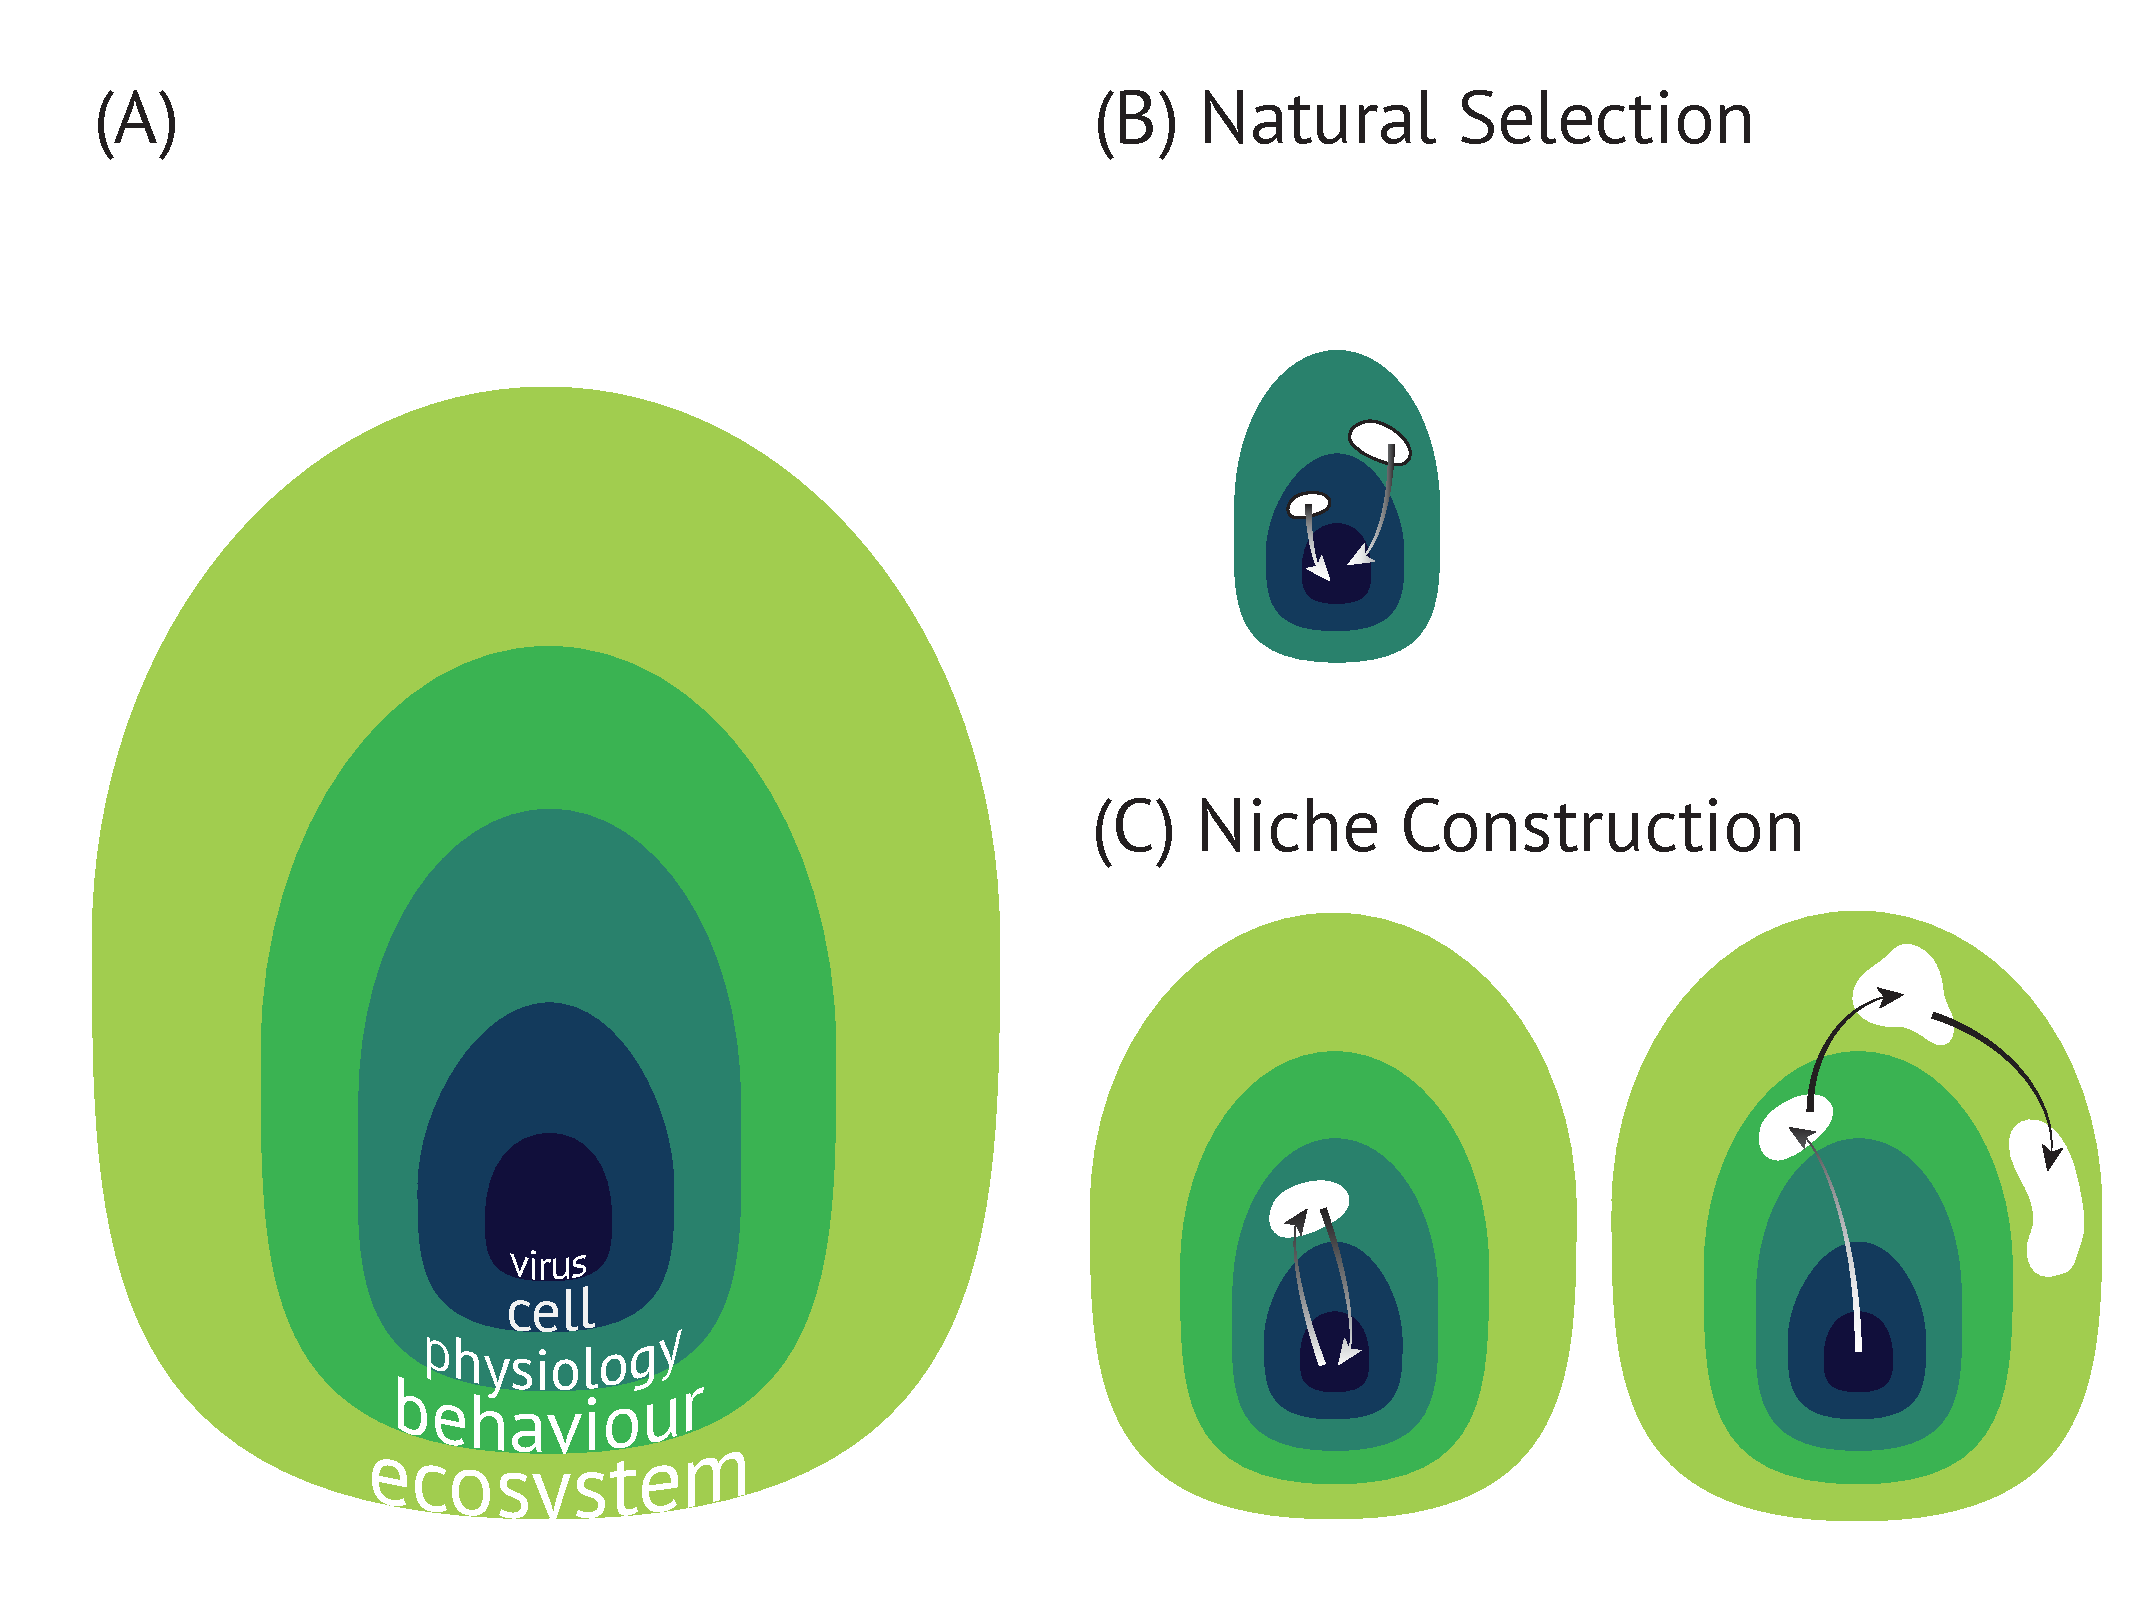
\includegraphics{Figures/VNC-02-Figure1.pdf}
\caption{Schematic depiction of niche construction as it applies to
viruses. In (A), viruses interact with their environments (the host and
beyond) on multiple nested levels. At the level of the host, the virus
can affect the host's cells, physiology, and behaviour. Beyond the focal
host, viruses can affect the broader ecosystem. This includes other
hosts and abiotic aspects of the environment (see text for more detail).
Under natural selection alone (B), viruses are understood to adapt to
the environment, not the other way around. Niche construction in viruses
(C) operates across and within levels to generate selective feedback.
Evolutionary studies of viruses have tended to focus on the first two
levels of the cell and the host's physiology. Under niche construction
viruses modify their environment and modified selection pressures then
feedback to the virus and/or other organisms.}
\end{figure}

\begin{center}\rule{3in}{0.4pt}\end{center}

\section{Glossary}\label{glossary}

\textbf{Commensalism}: a relationship between organisms in which one
benefits without harming or helping the other(s). Viruses that persist
in their host without causing disease or other detrimental effects to
the host (i.e.~viruses that escape immune surveillance) would be
commensal.

\textbf{Horizontal transmission}: transmission between contemporaries in
the same generation, such as the spread of influenza between humans via
contact or sneezing.

\textbf{Mutualism}: a relationship between organisms in which all
partners benefit.

\textbf{Niche construction}: an evolutionary process in which organisms
modify their environments and so modify their own and others' selection
pressures. See Box 1 for a detailed introduction to niche construction.

\textbf{Obligate intracellular parasite}: intracellular parasites are
those which grow and reproduce inside host cells. Viruses cannot
reproduce without the machinery for protein synthesis inside of the host
cells, and so are reliant (obligated) on those cells.

\textbf{Parenteral transmission}: transmission of an infectious agent
that occurs intravenously, for example through blood transfusions or
intravenous drug use.

\textbf{Pathogen}: broadly, an infectious agent that causes disease.
Pathogens include prokaryotes (e.g.~bacteria), eukaryotes (e.g.~fungi),
and subcellular agents (viruses, prions).

\textbf{Transmission}: passing of an infectious agent from one
individual to another. Viruses are transmitted by a number of routes,
such as physical contact, fecal-oral via contaminated food or water, or
via airborne transmission. Transmission can also involve an intermediate
host or a vector (an agent, such as a mosquito, that carries the
pathogen from one host to another).

\textbf{Vertical transmission}: transmission from parent to offspring,
usually through the germ line of an infected individual.

\textbf{Virulence}: Here we define virulence to mean the ability of a
pathogen species to cause disease, and in particular the increased death
rate of a host due to the disease.

\begin{center}\rule{3in}{0.4pt}\end{center}

\section{Why niche construction is important to
viruses}\label{why-niche-construction-is-important-to-viruses}

Viruses are exemplars of rapid evolutionary change, with small genomes,
massive population sizes and error-prone replication (especially in RNA
viruses) allowing for fast and relatively wide exploration of sequence
space \citep{Duffy:2008qy}. The viral literature has emphasized
straightforward environmental pressures (natural selection) as a cause
of viral evolutionary change, usually immune pressures such as the
yearly sequence evolution of influenza \citep[e.g.][]{Watanabe:2012ve}.
Yet there is growing recognition that disease-causing viruses, while
salient, are only a part of the organismal virome \citep{Lecuit:2013jk}.
Together with the complex effects that viruses can have on hosts and
beyond the host, there is a need for a comprehensive study of the
network of evolutionary processes in which viruses are embedded. We
suggest a new way to view viral interactions with the host on four
levels of organisation (Figure 1). These levels are the effects on the
host's cells, physiology (e.g.~fever as a result of infection), the
host's behaviour (e.g.~aggression due to viruses such as rabies or borna
virus), and the broader ecosystem \citep[e.g.~marine viruses affecting
global CO\textsubscript{2};][]{Suttle:2007fv}. Evolutionary studies of
viruses, such as the deep literature on transmission / virulence
trade-offs, have tended to ignore these higher level effects on host and
ecosystem. By focusing on biases in selection that emerge from changes a
virus makes to its environment, niche construction can provide a
parsimonious and comprehensive explanation of complex interactions that
bridge viral evolution and ecology \citep{Matthews2014}.

Following this, an illuminating aspect of viral niche construction that
is problematic under standard evolutionary theory is the difference in
reproductive timescale between a virus and its host(s). Viral
replication speed and population growth means that multiple generations
pass before the host responds at the level of physiology or behaviour,
and many more generations pass before effects are felt by the virus or
other organsisms at the level of the ecosystem. This difference in
timescale suggests that many host and ecosystem responses to viral
manipulations are experienced as `environment' from the perspective of
the virus. Viruses present at the beginning of an infection may
experience a dramatically different selective environment than viruses
involved in transmission because of changes to host physiology or
behaviour (e.g.~increased opportunity for transmission in rabies), or in
infections inspired in hosts affected by the gradually-accumulated
ecosystem effects of the virus (e.g.~marine viruses affecting global
ocean and atmospheric CO\textsubscript{2} levels). Coevolution under
standard evolutionary theory requires, by definition, reciprocal
evolutionary change \citep{Matthews2014}; one organism causes
evolutionary change in another, and in doing so results in evolutionary
change to themselves. Viruses often result in significant changes in
their hosts or ecosystems that result in evolutionary change to the
virus but not the host. A host infected with rabies (Figure 2A) does not
experience evolutionary change from the change in its behaviour (or does
not do so on the same timescale experienced by the local viral
population), but the virus experiences modified selection through the
infection and across infections by its environmental modification. We
argue that this is one way in which niche construction provides novel
insights into viral evolution.

Odling-Smee et al. \citep{Odling-Smee:2013zr} (Table 1) list twelve
insights derived from a niche construction perspective, and many of
these apply to viruses. For instance, niche construction can lead to
fixation of genotypes or phenotypes that would otherwise be deleterious
or neutral, and many viral mutualisms are likely to be driven by this
mechanism. As an example of this, panic grasses (\emph{Dichanthelium
lanuginosum}) that grow in geothermal soils in Yellowstone National
Park, USA co-exist with a fungal endosymbiont (\emph{Curvularia
protuberata}) that it requires to survive. The fungus allows the grasses
to grow in soils with temperatures greater than 50°C. However, it has
been discovered that the fungus relies on a virus (Curvularia
thermal-tolerance virus, or CTV) to provide this thermal tolerance;
fungi cured of the virus do not provide this service to their host
grass.

\section{Candidate niche-constructing
viruses}\label{candidate-niche-constructing-viruses}

To illustrate the concepts in the previous sections, we draw from the
virological literature to non-exhaustively survey candidates for viral
niche construction. Note that we are suggesting systems for which niche
construction might be a useful perspective; both theoretical and
empirical work is required to demonstrate that these are traits
maintained or promoted by niche construction.

\begin{figure}[htbp]
\centering
\includegraphics{Figures/VNC-02-Figure2.pdf}
\caption{Conceptual niche construction pathways in viruses. In this
diagram, solid lines indicate time while dashed lines are evolutionary
processes, black for natural selection and grey for niche construction.
A population of rabies virus, P(1) (top), causes encephalitis by
modifying cells in the central nervous system (cells/physiology) and
affects the host behaviour. This is depicted as the change in host state
from time 1, H(1), to time 2, H(2). The host's increased aggression
creates a new selective condition for the virus at time 2, P(2), in
terms of increased transmission through salivary transmission.
Rinderpest (bottom) caused a high death rate among artiodactyl host
populations at time A(1) and wiped out entire populations by time 2,
A(2), causing effects that rippled throughout the broader ecosystem.
This would have created new selective conditions for the virus itself as
well as other organisms in the ecosystem (see text for details).}
\end{figure}

Many viruses have effects centring on host cells and physiology. For
instance, mammalian viruses have evolved several strategies to
manipulate the important Pl3K-Akt-mTOR signalling pathway in cells,
affecting broad targets in cellular metabolism, growth, synthesis, and
translation \citep{Buchkovich2008}. Retroviruses, especially endogenous
retroviruses (ERVs), fit well into this category. Retroviruses such as
HIV use reverse transcription to transcribe their RNA genomes into DNA
which is then integrated into the host genome and undergoes normal
cellular transcription and translation to replicate further. Endogenous
retroviruses continue this by integrating into the host genome and
passing vertically through the germline from parent to offspring,
usually losing their ability to replicate. These modifications of the
host genome on a temporary or permanent basis can shift host-virus
interactions from antagonistic to commensal or even mutualistic. One
striking example of this is placental ERVs \citep{Haig:2012qf}, which
likely evolved placental expression to allow vertical transmission of
the virus, and in turn had their envelope proteins co-opted to develop
mammalian placentas. This has occurred independently in multiple
mammalian lineages \citep{Lavialle:2013oc}, making this a reasonable
candidate example of niche construction.

Another example of cellular and physiological modification working
together comes from Polydnaviruses (PDV), which integrate into the
genomes of ichneumonid and braconid parasitoid wasps
\citep{Roossinck:2011iz}. These viruses replicate in wasp ovaries and
are injected into the wasp's host along with its egg. Virus-free eggs
are encapsulated by the caterpillar host in a structure that prevents
the egg from developing, but the PDV carried by the wasp carries genes
to suppress this immune response. Experimental work has shown that eggs
do not survive without the viral genes. Niche construction linking host
physiological manipulations to transmission benefits in this way is
likely common. For example, Norovirus causes severe vomiting and
diarrhea and rhinovirus causes sneezing and coughing; both physiological
manipulations receive feedbacks from dramatically increased
transmission.

Niche construction acting at the level of the cell may even change the
transmission route of a viral group. Flaviviruses are arthropod-borne
viruses that replicate and cause disease in vertebrates and are usually
spread by their arthropod vectors. However, insect-specific flaviviruses
such as \emph{Culex} flavivirus have evolved to spread directly within
their arthropod hosts (parent to offspring) through eggs without
requiring an intermediate vertebrate host \citep{Bolling:2012fp}.
Phylogenetic analyses of the flaviviruses suggest that this modification
to insect-specific forms may have occurred multiple times, as there is
no evidence of host-virus co-divergence, and resulted in multiple
host-switching events \citep{Cook:2012gt}. Similar processes may
interact with the effect of the virus on the host to modify viral
selection pressures. For example, it is known that murine norovirus can
shift between chronic and acute infection with a single point mutation
in the NS1/2 protein \citep{Borin2013}. Understanding the process of
niche construction between effects on the host's physiology and
subsequent viral transmission may help explain these changes.

Viruses also engage in powerful manipulations of host behaviour, which
often feed back into selection on their transmission or virulence or
into selection pressures on other organisms. The neurotropic RNA virus
rabies (of the \emph{Rhabdoviridae} family) causes encephalitis in the
central nervous system of its animal hosts \citep{Schnell:2010ve} that
may result in large increases in aggression and aid in transmission
through saliva. Niche construction can lead to the promotion and
maintenance of these traits together by causing the first host
manipulation (either the behavioural manipulation or transmission
through saliva) to viral fitness when it acquires the second trait.
Separately, they are difficult to explain; a placid animal transmitting
through saliva does not aid viral fitness, and increased aggression does
not benefit the virus without salivary transmission. However, a
protovirus causing aggression and biting as a side-effect of CNS
infection would have made the acquisition of salivary transmission
extremely valuable. Seoul virus (family \emph{Bunyaviridae}), which
causes increased aggression in male Norway rats \citep{Klein:2004tg} and
is spread through bite wounds via saliva \citep{Hinson:2004uq}, may be a
result of a similar niche construction process. Borna virus (family
\emph{Bornaviridae}) also causes increased aggression in multiple host
species from horses to dogs \citep{Kinnunen:2013cy}, but here the method
of transmission is not known with certainty.

Niche construction by viral manipulation of aggression is not limited to
traits which transmit through biting. For instance, Kakugo virus is a
picorna-like RNA virus that infects European honeybee (\emph{Apis
mellifera L.}) workers in Japan and causes significant increases in
aggression. It has been suggested that this virus is responsible for the
aggressive defense of European honeybee colonies against attacking Asian
giant hornets (\emph{Vespa mandarinia japonica})
\citep{Fujiyuki:2005nx}. Since Kakugo is likely transmitted by mites of
the genus \emph{Varroa} \citep{Fujiyuki:2006od}, this implies that the
virus feeds back into host colony survival and the virus' transmission
simultaneously. Though Kakugo has been found to a limited extent in
North America \citep{Bromenshenk:2010vn}, we can find no reports of such
aggression in colonies outside Japan.

More speculatively, we can predict other niche-constructed behavioural
manipulations that modify transmission. Aggression associated with
strongly pathogenic viruses like rabies is easily spotted and consistent
with a bias for disease-causing viruses \citep{Lecuit:2013jk}, but many
parasites manipulate social behaviour such as mating and social rank
\citep[e.g.][]{Klein:2003lr}. Niche construction predicts that viruses
manipulating sociality to enhance their transmission are possible, such
as a sexually-transmitted virus modifying hormone production; such
viruses will likely be vertically or sexually transmitted and weakly
pathogenic, commensal or even mutualistic.

Viruses also drive large-scale population dynamics that contribute to
niche construction processes for other organisms. One powerful example
comes from bacteriophage-mediated virulence factors. The virulence of
many pathogenic bacteria is enhanced by phages, and others even require
phages to cause disease (reviewed in \citep{Wagner:2002wb}).
\emph{Escherichia coli} and \emph{Pseudomonas aeruginosa}, for instance,
adhere to buccal epithelial cells and are enhanced by phage infection
(e.g.~phage FIZ15 for \emph{P. aeruginosa}; see Table 1 of
\citep{Wagner:2002wb}). Phages also confer enhanced invasion, resistance
to serum- and phagocyte-mediated innate immunity, and even antibiotic
resistance. Some bacterial pathogens also rely on phages for production
of toxins, such as \emph{V. cholerae}, which only produces toxin when
genes are transferred from a lysogenic phage known as CTXΦ
\citep{Wagner:2002wb}. There is evidence that this act of viral niche
construction affects not only cholera transmission (through diarrhea
\citep{Wagner:2002wb}), but may also drive seasonal cholera epidemics in
humans \citep{Faruque:2005gl}. The interplay of viral and bacterial
population dynamics would create fluctuating selection pressures in both
organisms. Similarly, it is known that bacteriophages follow and even
drive the population dynamics involved in periodic cyanobacterial blooms
\citep{Bratbak:1990pi}. Yoshida et al. \citep{Yoshida:2008zp} describe
the association of cyanophages with the bloom-forming cyanobacteria
\emph{Microcystis aeruginosa}; some strains of \emph{M. aeruginosa}
produce potent hepatoxins called microcystins that are responsible for
poisoning humans and other animals. Any regulation of bacterial
populations by cyanophages in this system is likely to have selective
effects on surrounding populations that can be studied.

Viral modifications of host cells or physiology can even have profound
effects on the ecosystem at large. Just as beavers building a dam will
influence selection on organisms in the surrounding ecosystem
\citep{Odling-Smee:2003fk}, viruses causing widespread population losses
can significantly affect selection pressures experienced by other
organisms. For example, rinderpest (Figure 2) is an RNA virus that
produced a panzootic outbreak wiping out nearly every artiodactyl (cows,
pigs, sheep, wildebeest, giraffe, gazelle, etc.) in Ethiopia and caused
the Great Ethiopian Famine of the late 19th century
\citep{Morens:2011qf}. This massive population loss caused knock-on
effects throughout the region; as described in \citep{Morens:2011qf}, a
sudden lack of fertilizer (cow dung) brought planting and harvesting to
a halt, led to an explosion in rat, locust, and caterpillar populations,
encouraged smallpox outbreaks and killed as much as one-half to
two-thirds of human populations in affected areas of East Africa. The
disruption to the Eastern African ecosystem almost certainly changed
selective pressures for a wide variety of organisms in the region,
including the virus itself as host populations disappeared. A number of
examples of disease-induced extinction have been observed
\citep{Castro:2005vn}, and from a niche construction perspective we
predict that viruses will be important drivers of population dynamics in
many host and non-host species, often with consequences that affect the
virus itself.

On a global scale, marine viruses are responsible for significant
horizontal transfer of core photosynthetic genes for cyanobacteria (host
to phage, phage to host, and phage to phage: \citep{Sullivan:2006fk}).
Along with this, Thompson et al. \citep{Thompson:2011cr} argue that
cyanophages actually redirect host metabolism by the use of host-like
metabolic genes in order to force the host to process carbon. This would
allow the phage to increase the production of deoxynucleotides and
increase replication by manipulating the cellular environment. Together
with the potential upregulation of host photosynthesis by cyanophages
\citep{Lindell:2007pi} and the role of viruses in the `biological pump'
which increase the rate of CO\textsubscript{2} build-up in the
atmosphere \citep{Suttle:2005bs}, the combined effects on marine
photosynthesis and the global carbon may be highly significant (as in
the example of earthworms above).

\section{Why viruses are important to niche construction
theory}\label{why-viruses-are-important-to-niche-construction-theory}

While niche construction theory has been enthusiastically received in
evolutionary biology \citep{Laland:2010gb, Odling-Smee:2013zr}, it has
been critcised on the grounds that theory has run ahead of empirical
tests \citep{Scott-Phillips2014}. Viruses offer a compelling testbed for
identifying and manipulating niche construction pathways because they
evolve quickly and have small genomes, making it easy to identify and
study their molecular pathways. Matthews et al. \citep{Matthews2014}
call for experimental tests and a framwork under which to conduct them,
and we argue that viruses present many powerful candidates for tests of
niche construction (previous section).

An explicit example of the potential for new empirical work on niche
construction comes from \emph{Baculoviridae}, a family of invertebrate
viruses that infect arthropod hosts. This virus causes a pathology in
caterpillars known as ``tree-top disease'', in which the virus
manipulates infected caterpillars to the top of its host foliage and
liquefies the caterpillar after it dies from infection
\citep{Hoover:2011ly}. With experimental work demonstrating the genetic
mechanisms underlying this effect
\citep[e.g.][]{Hoover:2011ly, Hawtin:1997uq} and a mathematical model
that provides hypothesised a potential pathway for niche construction to
promote and maintain these traits in Baculovirus \citep{Hamblin:2013fk},
the stage is set for experimental manipulations to test niche
construction as described in \citep{Matthews2014}. For instance, if the
baculovirus-host system were modified so that the behavioural
manipulation of the caterpillar was suppressed, removing the
transmission advantage from liquefying the host on top of its foliage,
we could predict that either or both traits would be quickly lost (and
in fact, we know that plaque-derived cultures of these viruses almost
always lose a gene associated with the manipulation
\citep{Erlandson:2009ve}; this phenomenon remains to be shown
experimentally).

\section{Concluding remarks}\label{concluding-remarks}

The evolutionary study of viruses has a rich and productive history
including bodies of theory and experiment on transmission and virulence,
immune system coevolution, and epidemiological modelling. However, with
new understandings of viral diversity and the often complicated
interactions between virus and host has come the realisation that
pathogenic viruses are only one part of the global virome and that
viruses of all kinds can have sweeping effects on hosts, populations,
and even globally. We believe that niche construction theory is a useful
and practical lens through which to explain and unify these diverse
phenomena into a cohesive and productive framework for theory alike. We
also believe that virology and niche construction theory have much to
offer each other; NCT offers a useful approach to the study viral
evolution, and virology offers NCT many flexible experimental systems
with which to put theory to the test.

\section{Acknowledgments}\label{acknowledgments}

This work was supported by Australian Research Council Discovery Grant
DP110100465.

\clearpage
\bibliography{VNC-02-abbrev}

\listoffigures

\end{document}